%%%%%%%%%%%%%%%%%%%%% Chapter 11 %%%%%%%%%%%%%%%%%%%%%%%%%%%%%%%%%
% Adversarial Hardening: Defending Against Evasion
%%%%%%%%%%%%%%%%%%%%%%%%%%%%%%%%%%%%%%%%%%%%%%%%%%%%%%%%%%%%%%%%%
\motto{A model that is private but fragile is a model that cannot be deployed. Trustworthy AI must survive even under adversarial conditions.}

\chapter{Adversarial Hardening: Defending Against Evasion}
\label{chap:adversarial_hardening}

\abstract{This chapter addresses the internal robustness of AI models against adversarial perturbations. We define the concept of evasion attacks, where imperceptible changes to input data can cause a model to fail spectacularly. We analyze the mechanisms behind these attacks, such as the Fast Gradient Sign Method (FGSM), and explore defensive strategies including adversarial training, defensive distillation, and certified robustness through randomized smoothing. Ensuring that a model degrades gracefully under noise is a core requirement for safety-critical deployment.}

\section{The Fragility of Deep Learning}
\label{sec:fragility}

Modern neural networks are remarkably accurate on average, but they are also remarkably fragile. A well-known phenomenon in AI research is the \textbf{Adversarial Example}: an input to a machine learning model that is specifically designed by an attacker to cause the model to make a mistake.

In image classification, this often takes the form of "noise" that is imperceptible to the human eye but causes a model to classify a "Panda" as a "Gibbon" with 99\% confidence. In the context of the Trustworthy AI Architect, this is not just a curiosity; it is a security threat. A traffic sign recognition system in an autonomous vehicle or a facial recognition system in a secure facility must be hardened against such evasion attacks.

\begin{figure}[h]
\centering
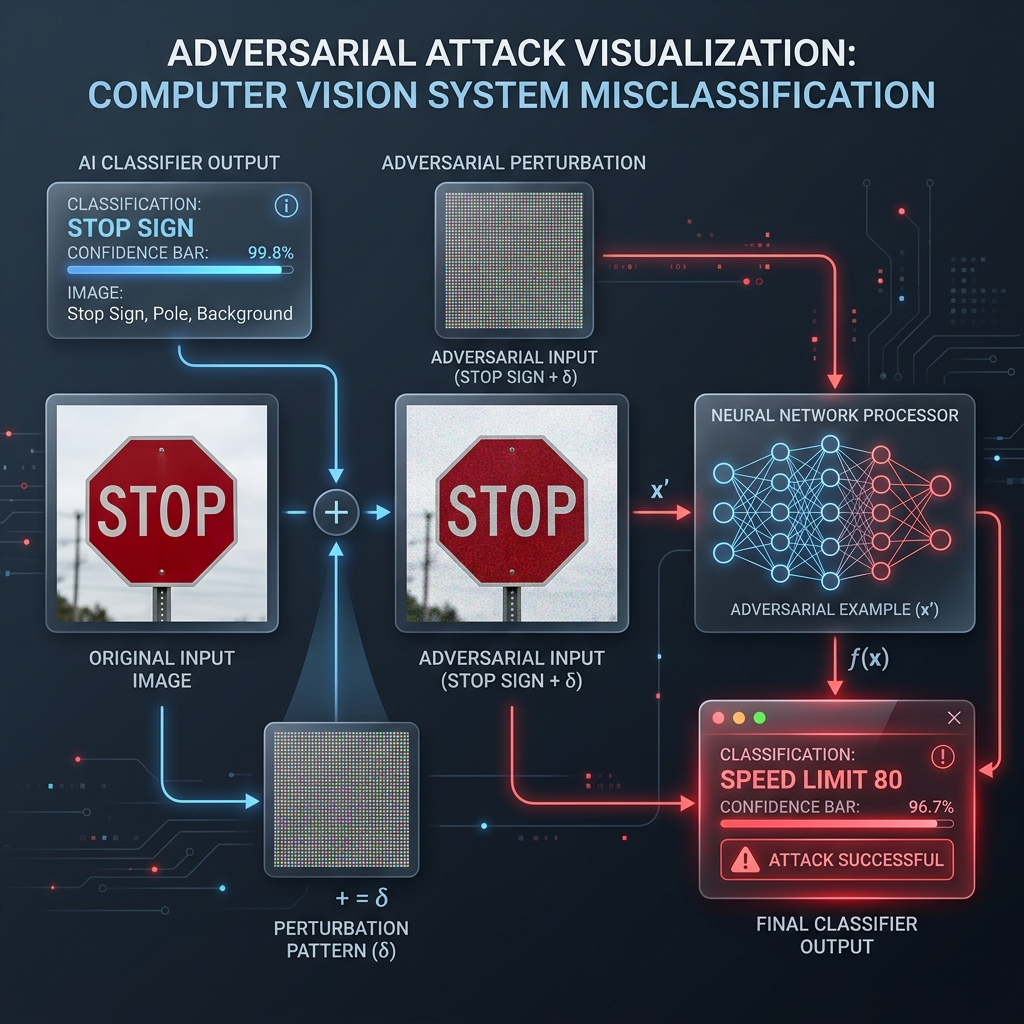
\includegraphics[width=\textwidth]{figures/ch11_adversarial.png}
\caption{Adversarial Attack Visualization: A subtle perturbation added to a Stop Sign input causes the AI classifier to predict 'Speed Limit 80' with high confidence.}
\label{fig:ch11_adversarial}
\end{figure}

\section{Evasion Attacks: FGSM and Beyond}
\label{sec:evasion_attacks}

The most common way to generate adversarial examples is to use the model's own gradients against it. The \textbf{Fast Gradient Sign Method (FGSM)} is a classic example:

\begin{equation}
x_{adv} = x + \epsilon \cdot \text{sign}(\nabla_x J(\theta, x, y))
\end{equation}

By moving the input $x$ in the direction of the gradient of the loss function $J$, the attacker maximizes the model's error with the smallest possible perturbation $\epsilon$.

\section{Defensive Strategies}
\label{sec:defensive_strategies}

To build a robust model, the architect has several defensive maneuvers:

\begin{description}
  \item[Adversarial Training:] 
        The most effective defense is to include adversarial examples in the training set itself \cite{goodfellow2014}. By training the model to correctly classify perturbed inputs, we force it to learn more robust features.
  \item[Defensive Distillation:]
        This technique involves training a model to predict the "softened" output labels of a teacher model, reducing the sensitivity of the gradients and making it harder for an attacker to find effective perturbations.
  \item[Certified Robustness:]
        For high-stakes applications, we seek a mathematical guarantee of robustness. \textbf{Randomized Smoothing} is a popular technique that adds noise to the input during inference and uses a statistical "majority vote" to certify that the prediction will remain constant within a certain radius of the input \cite{cohen2019}.
\end{description}

\section{Conclusion}
\label{sec:conclusion_hardening}

Adversarial hardening ensures that our models are not just "fair-weather" performers. By making robustness a primary architectural requirement, we ensure that our AI remains reliable in the face of environmental noise and active manipulation. In the next chapter, we look at how to make these robust decisions transparent and explainable through the \textbf{Explainability Stack}.


